\documentclass[11pt]{article}
\usepackage[T1]{fontenc}
\usepackage{lmodern}
\usepackage{amsmath, amssymb}
\usepackage{booktabs}
\usepackage{graphicx}
\usepackage{natbib}
\usepackage[margin=1in]{geometry}
\usepackage{microtype}
\usepackage{array}
\usepackage{setspace}
\usepackage{xcolor}
\usepackage{hyperref}
\usepackage{cleveref}
\hypersetup{colorlinks=true, linkcolor=blue!50!black, citecolor=blue!50!black, urlcolor=blue!50!black}
\setstretch{1.15}
% Generated by src/cvr/paper_numbers.py -- do not edit by hand.
\newcommand{\FirstYear}{2010}
\newcommand{\LastYear}{2023}
\newcommand{\IOLastYear}{2022}
\newcommand{\GDPLast}{32.4}
\newcommand{\DVRLast}{92.4\%}
\newcommand{\FVLLast}{7.6\%}
\newcommand{\FVLLastEUR}{2.48}
\newcommand{\DVRMin}{92.4\%}
\newcommand{\DVRMax}{95.8\%}
\newcommand{\DVRMinYear}{2023}
\newcommand{\DVRMaxYear}{2020}
\newcommand{\FVLMin}{4.2\%}
\newcommand{\FVLMax}{7.6\%}
\newcommand{\OfficialOutMin}{67\%}
\newcommand{\OfficialOutMax}{172\%}
\newcommand{\OfficialOutLast}{108\%}
\newcommand{\OfficialOutLastEUR}{34.9}
\newcommand{\GNILastEUR}{29.0}
\newcommand{\OFCPaidTwentyTwo}{22.3}
\newcommand{\OFCPaidLast}{29.2}
\newcommand{\NonSPEFDILast}{19.0\%}
\newcommand{\NonSPEFDILastEUR}{6.2}
\newcommand{\TotalFDIPaidLastEUR}{30.7}
\newcommand{\FOCLast}{22.0\%}
\newcommand{\FOCFirst}{8.5\%}
\newcommand{\FCredLast}{7.6\%}
\newcommand{\FLILast}{1.3\%}
\newcommand{\FATSForeignGOSLast}{2.76}
\newcommand{\DVRConsLast}{91.6\%}
\newcommand{\DVRTwentyTwenty}{95.8\%}
\newcommand{\DVRTwentyTwentyTwo}{93.8\%}
\newcommand{\MechFDI}{1{,}424}
\newcommand{\MechLabour}{182}
\newcommand{\MechOther}{454}
\newcommand{\MechPortfolio}{2}
\newcommand{\MechGov}{197}
\newcommand{\MechEU}{74}
\newcommand{\MechDebt}{145}
\newcommand{\MechFDIShare}{57\%}
\newcommand{\RecOneName}{Greece}
\newcommand{\RecOneEUR}{336}
\newcommand{\RecTwoName}{Offshore financial centres}
\newcommand{\RecTwoEUR}{270}
\newcommand{\RecThreeName}{United States}
\newcommand{\RecThreeEUR}{152}
\newcommand{\RecFourName}{Canada}
\newcommand{\RecFourEUR}{137}
\newcommand{\RecFiveName}{France}
\newcommand{\RecFiveEUR}{104}
\newcommand{\RecUnknownEUR}{1{,}083}
\newcommand{\RecUnknownShare}{44\%}
\newcommand{\RecConfEUR}{285}
\newcommand{\RecWorldEUR}{798}
\newcommand{\WorldUnallocMin}{378}
\newcommand{\WorldUnallocMax}{798}
\newcommand{\IndOneName}{Banking}
\newcommand{\IndOneEUR}{653}
\newcommand{\IndOneDVR}{68.5\%}
\newcommand{\IndTwoName}{Publishing (incl. software)}
\newcommand{\IndTwoEUR}{227}
\newcommand{\IndTwoDVR}{79.8\%}
\newcommand{\IndThreeName}{IT and information services (technology)}
\newcommand{\IndThreeEUR}{175}
\newcommand{\IndThreeDVR}{87.4\%}
\newcommand{\GovPeak}{284}
\newcommand{\GovPeakYear}{2016}
\newcommand{\GovTwentyTwo}{141}
\newcommand{\GovLast}{197}
\newcommand{\FIEFirst}{28.2\%}
\newcommand{\FIELast}{50.2\%}
\newcommand{\TICFirst}{21.4\%}
\newcommand{\TICLast}{40.7\%}
\newcommand{\ImpInterFirst}{4.8}
\newcommand{\ImpInterLast}{18.7}
\newcommand{\ImpGrowthTotal}{13.9}
\newcommand{\ImpGrowthFour}{8.7}
\newcommand{\FIEIT}{76\%}
\newcommand{\FIEAuxFin}{81\%}
\newcommand{\FIEPub}{72\%}
\newcommand{\FIEBank}{56\%}
\newcommand{\FIERest}{25\%}
\newcommand{\FIEConstr}{20\%}
\newcommand{\FIERetail}{32\%}
\newcommand{\PERestHome}{71}
\newcommand{\PERestAbroadVA}{2}
\newcommand{\PERestImp}{25}
\newcommand{\PERetailHome}{78}
\newcommand{\PERetailAbroadVA}{3}
\newcommand{\PERetailImp}{19}
\newcommand{\PEITHome}{26}
\newcommand{\PEITAbroadVA}{4}
\newcommand{\PEITImp}{70}
\newcommand{\PEBankHome}{40}
\newcommand{\PEBankAbroadVA}{7}
\newcommand{\PEBankImp}{48}
\newcommand{\PEConstrHome}{59}
\newcommand{\PEConstrAbroadVA}{1}
\newcommand{\PEConstrImp}{37}
\newcommand{\PERealEstHome}{89}
\newcommand{\PERealEstAbroadVA}{2}
\newcommand{\PERealEstImp}{8}
\newcommand{\EconDomVA}{26{,}301}
\newcommand{\EconImp}{18{,}677}
\newcommand{\ImpSrcOneName}{Russia}
\newcommand{\ImpSrcOneEUR}{2.1}
\newcommand{\ImpSrcTwoName}{Ireland}
\newcommand{\ImpSrcTwoEUR}{1.2}
\newcommand{\ImpSrcThreeName}{United States}
\newcommand{\ImpSrcThreeEUR}{1.2}
\newcommand{\PlatHome}{3.98}
\newcommand{\PlatOwner}{1.96}
\newcommand{\PlatSuppAbroad}{0.16}
\newcommand{\PlatImp}{13.90}
\newcommand{\PlatLabour}{2.03}
\newcommand{\SensThetaSpreadPP}{2.0}
\newcommand{\SensDVRLow}{91.2\%}
\newcommand{\SensDVRHigh}{93.8\%}
\newcommand{\SensAllLow}{85.0\%}
\newcommand{\SensAllHigh}{93.8\%}
\newcommand{\SensOFCDVR}{92.1\%}
\newcommand{\SensBopUpperDVR}{86.4\%}
\newcommand{\SensBanksGrossDVR}{91.4\%}
\newcommand{\SensNoTaxDVR}{91.7\%}
\newcommand{\SensRhoNoneDVR}{91.7\%}
\newcommand{\SensRhoGrossDVR}{92.2\%}
\newcommand{\SensRhoNetDVR}{92.2\%}
\newcommand{\SensBanksGrossFirst}{86.9\%}
\newcommand{\DVRFirst}{94.6\%}
\newcommand{\LabourGrossLast}{230}
\newcommand{\SSCShareLast}{20.7\%}
\newcommand{\InterestRatioLast}{27\%}
\newcommand{\IntraShareLast}{33\%}
\newcommand{\IntraShareFirst}{17\%}
\newcommand{\InterestRatioFirst}{34\%}
\newcommand{\BankBopLast}{1{,}198}
\newcommand{\BankFatsLast}{640}
\newcommand{\BanksPaidFirst}{1{,}503}
\newcommand{\BanksRecvFirst}{2{,}065}
\newcommand{\BridgeSpeLast}{29.2}
\newcommand{\BridgeFdiEqOfficialLast}{2.63}
\newcommand{\BridgeFdiEqModelLast}{0.61}
\newcommand{\BridgeFdiEqGapLast}{2.02}
\newcommand{\ThetaN}{14}
\newcommand{\ThetaGroups}{10}
\newcommand{\ThetaMean}{0.90}
\newcommand{\FirmsN}{42}
\newcommand{\FirmsForeignUCI}{12}
\newcommand{\FirmsUnresolvedUCI}{21}
\newcommand{\CatalogueN}{96}
\newcommand{\GNIMaxGap}{0.008\%}

\newcommand{\EUR}{EUR~}

\title{Who Captures the Value Generated in Cyprus?\\[4pt]
\large A Recipient-Country Accounting of Domestic Value Retention and Foreign Leakage, \FirstYear--\LastYear}
\author{Diomides Mavroyiannis\thanks{Milestone Institute, Budapest. \href{mailto:dmavroyiannis8@gmail.com}{dmavroyiannis8@gmail.com}. Data, code and an interactive dashboard: \url{https://github.com/diomavro/country-value-retention}. All numbers in this paper are generated by the repository's pipeline from official sources; every figure can be traced to its source table.}}
\date{Data release v0.1, September 2026}

\begin{document}
\maketitle

\begin{abstract}
\noindent
In official statistics Cyprus pays abroad primary income---wages, profits, interest and dividends---worth between \OfficialOutMin{} and \OfficialOutMax{} of its GDP each year.
Most of it is income that only passes through Cypriot holding companies.
We ask a narrower question: of the value produced in Cyprus, how much accrues to residents, how much to the rest of the world, and to whom?
We split every euro of GDP by recipient and industry, combining CYSTAT's supply--use and input--output tables, statistics on foreign-controlled firms (FATS), the balance of payments by paying sector, and a hand-built ownership graph.
In \LastYear{} at most \DVRLast{} of Cypriot GDP accrued to residents (for the central foreign equity share); \FVLLast{} (\EUR\FVLLastEUR~bn) accrued abroad, \MechFDIShare{} of it as profits of foreign-owned firms.
Retention ranged from \DVRMin{} to \DVRMax{} over \FirstYear--\LastYear{} and has fallen since 2020.
A sector-by-sector bridge accounts for the difference from the official outflow.
Separately, the import content of final demand for Cypriot output rose from \TICFirst{} to \TICLast{} between \FirstYear{} and \IOLastYear{}.
\end{abstract}

\medskip
\noindent\textbf{Keywords:} national accounts; value added; foreign direct investment; special purpose entities; input--output; ownership networks; Cyprus.\\
\textbf{JEL:} E01, F23, F62, C67, O52.

\section{Introduction}
\label{sec:intro}

When a Cypriot restaurant pays a food-delivery platform a commission of \EUR20, how much of that money ends up abroad, and why?
A common answer is ``all of it, because the platform is foreign-owned.''
That is the wrong reason.
Ownership moves only the owner's profit abroad.
The rest of the commission pays Cypriot staff, Cypriot taxes and suppliers.
Some of those suppliers are Cypriot; others are abroad.
Revenue is not value, and a foreign owner has a claim on profit, not on revenue.

This paper applies that logic to a whole economy.
We ask: \emph{of the value generated by production in Cyprus, how much accrues to residents, and how much to other countries---through foreign workers, foreign owners, foreign lenders, and EU institutions?}
We also ask a companion question: \emph{of each euro spent on Cypriot output, how much pays for imported inputs, and from where?}

Cyprus is a demanding first case.
Its official accounts record primary income paid abroad of \EUR\OfficialOutLastEUR~bn in \LastYear{}, which is \OfficialOutLast{} of GDP (\EUR\GDPLast~bn).
In 2018--2021 the figure exceeded 150\% of GDP.
Taken at face value, Cyprus would be giving away more than it produces.
It is not.
Most of these flows are dividends and interest that Cypriot-registered holding companies receive from abroad and pass on to foreign owners, with little Cypriot production in between.
In 2022, financial corporations other than banks---the sector that contains Cyprus's special purpose entities (SPEs)---paid \EUR\OFCPaidTwentyTwo~bn of the investment income that left the country.
GNI, which nets these flows against receipts, was \EUR\GNILastEUR~bn in \LastYear{}.
Neither GNI nor the gross outflow answers our question, because both mix value produced in Cyprus with value produced elsewhere and routed through it.

We therefore build the accounting from the production side.
We start from GDP by industry and split each industry's value added into compensation of employees, taxes on production, and operating surplus.
Each outflow may draw only on its own kind of income.
Profits of foreign-owned firms come out of operating surplus, never out of wages or taxes, and pay to non-resident workers only out of compensation.
Profits of foreign-owned firms are measured from FATS, which reports the operating surplus of foreign-\emph{controlled} firms in Cyprus by industry and by the country of their ultimate controller.
From that surplus we deduct depreciation, interest and Cypriot corporate tax, and apply the share of equity held by non-residents, calibrated on company filings.
The result, $V[i,j,k,t]$, allocates every euro of Cypriot GDP in year $t$ and industry $k$ to one recipient $j$.
Every cell carries its source, method, status and confidence.

\paragraph{Findings.}
At most \DVRLast{} of Cyprus's \LastYear{} GDP accrued to residents.
Given the central assumptions (\cref{sec:robust}), it is an upper bound because any outflow the statistics miss is counted as retained.
The remaining \FVLLast{} (\EUR\FVLLastEUR~bn) accrued abroad: \EUR\MechFDI~m as profits of foreign-owned firms, \EUR\MechOther~m as interest paid by firms and households to other foreign lenders (banks' interest paid abroad was smaller than their receipts), \EUR\MechDebt~m as interest paid to foreign parent companies, \EUR\MechGov~m as interest on public debt, \EUR\MechLabour~m as pay to non-resident workers, and \EUR\MechEU~m as customs duties passed to the EU.
These are \emph{accruals}: profits that foreign owners reinvest in Cyprus still accrue to them, as in the balance of payments.
Retention ranged between \DVRMin{} (\DVRMinYear) and \DVRMax{} (\DVRMaxYear).
It fell from \DVRTwentyTwenty{} in 2020 to \DVRLast{} in \LastYear{} as the surplus of foreign-controlled firms grew.
The largest identified recipients in \LastYear{} were \RecOneName{} (\EUR\RecOneEUR~m), \RecTwoName{} (\EUR\RecTwoEUR~m), \RecThreeName{} (\EUR\RecThreeEUR~m) and \RecFourName{} (\EUR\RecFourEUR~m).
The countries are those of the ultimate controller of the paying firm.
\RecUnknownShare{} of the outflow cannot be assigned to a country because the statistics are confidential or published only as world totals; we report it as such.

Imports are a separate channel and are not part of GDP.
Between \FirstYear{} and \IOLastYear{}, imported intermediate inputs grew from \EUR\ImpInterFirst~bn to \EUR\ImpInterLast~bn.
IT services, banking, auxiliary financial services and publishing account for \EUR\ImpGrowthFour~bn of the \EUR\ImpGrowthTotal~bn increase.
The import content of final demand for Cypriot output, counting suppliers' suppliers, rose from \TICFirst{} to \TICLast{}.

\paragraph{What is new.}
None of the ingredients is new; the contribution is to join them.
Value-added-in-trade statistics say where value is \emph{produced}.
Foreign-affiliate statistics say which firms are foreign-\emph{controlled}.
The balance of payments says what crosses the border, but in a hub economy it is dominated by pass-through.
We combine them into one accounting with four properties.
It never counts an imported input and the foreign value embodied in it twice.
It never counts wages or taxes as foreign capital income, and it counts interest once.
It removes SPE income.
And it is reconciled line by line with the official outflow.
Every step is automated and published with its code.

\paragraph{What this paper does not claim.}
The accounting describes where income accrues.
It does not say whether foreign ownership raised or lowered Cypriot incomes: a foreign-owned hotel that sends \EUR1m of profit abroad may also employ workers who would otherwise earn less.
Leakage is an accounting concept, not a cost.

\Cref{sec:concepts} explains the concepts with a worked example, and \cref{sec:literature} places the work in the literature.
\Cref{sec:data,sec:method} describe the data and methods.
\Cref{sec:results,sec:bridge,sec:industry,sec:country,sec:valuechain} present results.
\Cref{sec:robust,sec:limits,sec:discussion} cover sensitivity, limitations and discussion.

\section{Conceptual framework}
\label{sec:concepts}

A handful of ideas carry the whole analysis.
We state each in plain terms first, with a small example; the numbers in this section are made up and do not enter the results.

\paragraph{Value added, not revenue.}
A bakery that sells \EUR100 of bread and buys \EUR40 of flour and \EUR10 of electricity has added \EUR50 of value.
Summing revenue across firms double counts the flour, once in the miller's sales and again in the baker's.
Summing value added gives GDP.
If the flour was imported, the \EUR40 paid for something produced abroad, but it is the foreign miller's value added, not ``leakage of the bakery''.

\paragraph{Three kinds of income.}
The bakery's \EUR50 is \emph{primary income}: income earned by taking part in production.
It pays three groups: workers (compensation of employees), the government (taxes on production, net of subsidies), and owners and lenders (gross operating surplus).
Say \EUR30, \EUR2 and \EUR18.

\paragraph{Residence, not nationality.}
``Foreign'' means \emph{not resident}, the rule of the national accounts and the balance of payments \citep{UN2009SNA,IMF2009BPM6}.
A Greek citizen who lives and works in Nicosia is a Cypriot resident, so their wage stays in Cyprus.
A worker who lives in Greece and comes for a short contract is not.
We never use citizenship or country of birth as a proxy for residence.
A company is resident where it is incorporated.

\paragraph{Owners get profit, lenders get interest.}
Operating surplus must first replace worn-out equipment (depreciation) and pay lenders (interest).
Cypriot corporate tax is due on what remains.
Only the rest is profit, and an owner's claim is its share of that profit.
In the bakery, take the \EUR18 of surplus, subtract \EUR5 of depreciation and \EUR3 of interest to a Cypriot bank, and apply 12.5\% tax: \EUR8.75 is left.
A foreign owner of 60\% of the shares has a claim on \EUR5.25, and the other \EUR44.75 of the \EUR50 stays in Cyprus.
Had the bakery borrowed from a German bank, the \EUR3 of interest would accrue to Germany.
It is counted once, as interest.
The same host-tax logic applies to workers: the part of a non-resident's pay that goes to Cypriot social insurance stays in Cyprus.

\paragraph{Accruing is not paying.}
If the foreign owner leaves its \EUR5.25 in the bakery to buy a new oven, the profit has still accrued to the owner.
The balance of payments records this as \emph{reinvested earnings}.
Our figures measure claims on value, not cash crossing the border in the year.

\paragraph{Following ownership up the chain.}
A Cypriot subsidiary may be owned by a Dutch holding company owned by a US parent.
Official statistics on foreign-controlled firms attribute a firm to its \emph{ultimate controlling institutional unit}: the unit at the top of the chain of majority control \citep{OECD2008BMD}.
We use that concept for recipient countries.
Where the records run out, we say \emph{unresolved} rather than invent a country.

\paragraph{The chain behind the chain.}
A restaurant imports olive oil directly and buys bread from a bakery that imports flour; the second import is indirect.
The input--output table records who buys from whom.
Its Leontief inverse $L=(I-A)^{-1}$ adds up suppliers, suppliers' suppliers, and so on \citep{Leontief1936,MillerBlair2009}.
Every euro of final spending on domestic output (valued before taxes on the final sale, such as VAT) is exhausted by three parts:
\begin{equation}
\underbrace{(v/x)\,L}_{\text{domestic value added}} \;+\; \underbrace{\mathbf 1' A_m L}_{\text{imported inputs}} \;+\; \underbrace{(t/x)\,L}_{\text{net taxes on products used as inputs}} \;=\; \mathbf 1'.
\label{eq:exhaust}
\end{equation}
Imports and value added are two slices of the same euro, so they cannot be double counted.

\paragraph{Two frames.}
\emph{Frame A} asks who receives the value added generated in Cyprus in a year: GDP minus what accrues to non-residents is retained.
\emph{Frame B} asks where a euro spent on a Cypriot product ends up: its Cypriot value added is routed through Frame A's recipient shares, and its imported inputs go to the countries that supplied them.

\paragraph{Why GNI is not the answer.}
GNI adds income residents earn abroad, which is value generated elsewhere.
And in a hub economy, primary income paid abroad includes income that SPEs receive from abroad and pass on.
Neither belongs in an account of value generated by Cypriot production.

\paragraph{Codes used in the paper.}
D1 compensation of employees; D12 employers' social contributions; D29--D39 other taxes on production net of subsidies; B2A3G gross operating surplus and mixed income (the income of the self-employed); CFC consumption of fixed capital (depreciation); NOS net operating surplus; S11 non-financial corporations; S12 financial corporations, of which S122 banks and S12M other financial corporations (where SPEs sit); S13 government; S1V firms and households; S2 the rest of the world.

\section{Related Literature}
\label{sec:literature}

This paper joins three literatures that measure the same object---the destination of value added generated on a territory---from different sides, and that have so far been kept apart.

The first is the input--output literature on value added in trade.
Building on \citet{Leontief1936} and the domestic/imported coefficient split in \citet{MillerBlair2009}, \citet{HummelsIshiiYi2001} measure the import content of exports, \citet{JohnsonNoguera2012} define value-added exports, and \citet{KoopmanWangWei2014} and \citet{LosTimmerdeVries2016} decompose gross exports into value-added and double-counted terms.
\citet{LosTimmerdeVries2015} show that the foreign value-added share of final manufactures has risen almost everywhere.
Surveys by \citet{Johnson2018} and \citet{AntrasChor2022} make clear that these measures, and the databases that implement them \citep{Timmeretal2015,Yamanoetal2021,Eurostat2019FIGARO,Ahmadetal2017}, attribute value added to the country where production takes place.
We borrow their double-counting logic but ask a different question: not where value is \emph{produced}, but who \emph{receives} it.

The second literature slices value chains by factor income.
\citet{Timmeretal2013} introduce ``GVC income'', \citet{Timmeretal2014} show that the capital share of value-chain income has risen, and \citet{TimmerMiroudotdeVries2019} document functional specialisation across countries.
\citet{ChenLosTimmer2018} attribute a large and growing residual to intangible capital and note that its location is recorded where intellectual property is registered.
This is exactly the case in a holding-company jurisdiction such as Cyprus, and it motivates the step these papers leave out: allocating capital income to the residence of its owner.

A closely related strand splits input--output tables by firm ownership.
The OECD AMNE database \citep{Cadestinetal2018} and \citet{MiroudotYe2020} separate value added of foreign affiliates from that of domestic firms.
Extended supply--use tables for the United States \citep{Fetzeretal2018} and the Netherlands \citep{Chongetal2019}, codified in \citet{UN2023GVC}, provide the compilation template we follow.
\citet{Lipsey2010} and \citet{CasellaBorgaWacker2023} warn that when intangibles and conduit FDI dominate, neither location nor immediate ownership identifies where production income accrues.
The ownership-split tables stop at foreign-\emph{controlled} value added.
They do not ask how much of it leaves the country, as distributed or reinvested earnings, or whether it only passes through on its way to a third country.

The third literature works from the residence side.
The SNA, BPM6 and the FDI benchmark definition \citep{UN2009SNA,IMF2009BPM6,OECD2008BMD} define the primary-income flows that bridge GDP and GNI.
\citet{Rassier2017} and \citet{Guvenenetal2022} show that profit shifting by multinationals distorts output, BoP and productivity by location.
Ireland's modified GNI* \citep{ESRG2016,FitzGerald2018} is the leading official response, but it is a single adjusted aggregate.
It does not decompose the leakage by sector or by recipient.
Our requirement that every euro of GDP be allocated to exactly one recipient is the cross-border counterpart of the distributional national accounts of \citet{PikettySaezZucman2018}.

Measuring these flows correctly requires dealing with special-purpose entities.
Investment-income flows are the counterpart of external positions \citep{LaneMilesiFerretti2018}, and those positions are heavily distorted by conduits.
\citet{DamgaardElkjaer2017} and \citet{DamgaardElkjaerJohannesen2024} estimate that a large share of global FDI is ``phantom'' investment in shell entities, and \citet{Casella2019} proposes a probabilistic look-through to ultimate investors.
\citet{BlanchardAcalin2016} and \citet{BolwijnCasellaRigo2018} show that hub FDI is largely pass-through.
\citet{Zucman2013} and \citet{Coppolaetal2021} demonstrate that restating external positions from residence to nationality changes bilateral patterns substantially.
Cyprus appears on the haven lists used to estimate shifted profits \citep{HinesRice1994,TorslovWierZucman2023}.
Related work quantifies profit shifting from FDI returns \citep{JanskyPalansky2019} and traces its footprint in the balance of payments \citep{HebousKlemmWu2021}.
Network studies of corporate control \citep{Vitalietal2011} classify Cyprus as a sink offshore financial centre \citep{GarciaBernardoetal2017}.
Russian round-tripping through Cyprus is documented by \citet{Ledyaevaetal2015} and \citet{RepousisLoisKougioumtsidis2019}, and IMF surveillance repeatedly flags the SPE-driven volatility of Cyprus's external accounts \citep{IMF2023CyprusSI,IMF2024Cyprus}.
We follow the IMF definition of SPEs \citep{SanchezMunozetal2022}, as applied by the Central Bank of Cyprus \citep{CBC2026External}, and use Eurostat's SPE split of FDI income together with a resident-sector rule.
This removes pass-through flows explicitly, instead of counting them either as domestic retention or as foreign capture.

Finally, for a tourism-intensive economy, the older tourism-leakage literature \citep{Sinclair1998} and recent work on platform intermediation \citep{RochetTirole2003,Hunoldetal2020,UNCTAD2019DER} point to a further channel.
A commission paid to a foreign-owned platform is often read as value captured abroad, but only the platform owner's share of profit is; the rest pays local staff, suppliers and taxes.
The accounting gives each part an explicit recipient.

Relative to these literatures, our contribution is integration rather than a new estimator.
We join the residence, ownership and value-chain layers into a single recipient-country by sector tensor.
The tensor adds up to GDP, is consistent with BPM6 primary income and FATS ownership, excludes double counting between imported-input leakage and foreign capital-income leakage, and is adjusted for SPEs.
Every cell is traceable to a published source.


\section{Data}
\label{sec:data}

All inputs are official statistics, downloaded by scripts and logged with URL, retrieval date and SHA-256 checksum in a catalogue of \CatalogueN{} datasets (\cref{app:data}).
Processing stops if a raw file no longer matches its checksum.
\Cref{tab:sources} lists the core sources.

\begin{table}[!htbp]
\centering
\small
\caption{Core data sources}
\label{tab:sources}
\begin{tabular}{>{\raggedright\arraybackslash}p{0.30\textwidth}>{\raggedright\arraybackslash}p{0.38\textwidth}>{\raggedright\arraybackslash}p{0.20\textwidth}}
\toprule
Source & Content used & Coverage \\
\midrule
CYSTAT supply--use and symmetric input--output tables (0640010E--0640055E) & domestic and imported intermediate use, 65 products; value-added components & 2010--2022 \\
CYSTAT sector accounts (0630030E) and Eurostat \texttt{nasa\_10\_nf\_tr} & rest-of-world primary income (D1, D2, D4); corporate depreciation, interest, employers' contributions & 2010--2024 \\
Eurostat \texttt{nama\_10\_a64} & GVA, compensation, depreciation, operating surplus by industry & 2010--2024 \\
Eurostat FATS (\texttt{fats\_activ}; \texttt{fats\_g1a\_08}) & operating surplus of foreign-controlled firms by industry and ultimate controlling country; before 2021 derived as value added minus personnel costs & 2010--2023 \\
Eurostat BoP (\texttt{bop\_c6\_a}, \texttt{bop\_rem6}, \texttt{bop\_fdi6\_inc}) & investment income by paying resident sector; compensation by partner; FDI income, total and SPE & 2010--2024 \\
Eurostat FIGARO (\texttt{naio\_10\_fcp\_ii*}) & supplying country of Cyprus's imported intermediates & 2010--2022 \\
Company filings (\FirmsN{} operating firms) & shareholders, parents, ultimate controllers & 2024--2026 \\
\bottomrule
\end{tabular}

\smallskip
\begin{minipage}{0.92\textwidth}\footnotesize
Notes: confidential cells (\ConfFatsLow{}--\ConfFatsHigh{} of FATS cells, \ConfFdi{} of FDI income cells up to \LastYear) are kept as missing, never set to zero.
Where a missing BoP cell leaves a flow unmeasured, the estimate is a lower bound on that flow and the omission is reported.
Full catalogue in \texttt{data\_catalogue.csv}.
\end{minipage}
\end{table}

Two features of the data shape the method.
First, the input--output tables are complete.
The symmetric tables contain no confidential cells and reconcile exactly to GDP and compensation in every year (\cref{app:method}).
Second, the balance of payments is dominated by pass-through.
In \LastYear{}, FDI income paid abroad was \EUR\TotalFDIPaidLastEUR~bn.
Excluding SPEs, as Eurostat publishes them, it was \EUR\NonSPEFDILastEUR~bn (\NonSPEFDILast{} of GDP).
Even that exceeds the operating surplus of all foreign-controlled firms in FATS (\EUR\FATSPublishedLast~bn; \EUR\FATSForeignGOSLast~bn with finance at the national-accounts level), because holding and trading companies with staff are not SPEs but still pass on foreign-earned income.
We therefore measure foreign-owned profit from the production side (FATS) and use the payments side as a comparator, bridged line by line in \cref{sec:bridge}.

\section{Methodology}
\label{sec:method}

\subsection{The recipient accounting (Frame A)}

For each industry $k$ and year $t$, the national accounts give $\text{GVA}_{k} = D1_{k} + D29X39_{k} + B2A3G_{k}$.
An outflow to country $j$ through mechanism $m$ is written $O^m_{jk}$.
Each mechanism may draw only on its own component, and never more than that component:
\begin{align}
\textstyle\sum_j O^{\text{labour}}_{jk} &\le D1_k, &
\textstyle\sum_{j,m\in\text{capital}} O^{m}_{jk} &\le \max(B2A3G_k,0),
\end{align}
and the pipeline stops if either bound is violated.
Retained value is the residual, $V[\text{CY},\text{CY},k] = \text{GVA}_k - \sum_{j,m} O^m_{jk}$, so $\sum_{j,k} V = \text{GDP}$ by construction.
This is an identity, not evidence of accuracy.
Taxes on products form a pseudo-industry.

\paragraph{Profits of foreign-owned firms.}
FATS reports gross operating surplus of foreign-controlled firms, before depreciation, interest and tax.
We use the finest published FATS code for each industry: for example publishing (J58) or IT services (J62--J63), and before 2021 every 2-digit division.
Only a section's unpublished remainder is split across its industries in proportion to operating surplus.
We then deduct depreciation ($c$) and interest paid ($\rho$), both per euro of gross operating surplus of non-financial corporations.
We use corporate ratios, not industry ratios, because industry surplus also includes the income of the self-employed.
For $\rho$ we use the interest non-financial corporations pay, after the national-accounts adjustment for bank services (FISIM), per euro of their surplus.
We do not net interest received: receipts from abroad are not value generated in Cyprus, and netting would credit them to foreign owners.
Actual interest before the FISIM adjustment is much higher in the post-crisis years, because domestic firms were heavily indebted: applied to all foreign-controlled firms it would leave them no or almost no profit in 2010--2015 and 11--29\% of surplus in 2016--2020 (in 2021--2023 it is close to, and in 2023 below, the central ratio).
We report it, the net-of-receipts version and $\rho=0$ as variants (\cref{sec:robust}); the year-by-year ratios are in \cref{app:method}.
We apply the statutory corporate tax rate $\tau_t$ and multiply by $\theta$, the non-resident share of equity:
\begin{equation}
O^{\text{FDI}}_{jk} = \text{GOS}^{\text{FATS}}_{k}\,(1-c-\rho)\,(1-\tau_t)\,\theta\,\sigma_{s(k),j}.
\label{eq:fdi}
\end{equation}
On this basis $\rho$ was \InterestRatioFirst{} in \FirstYear{} and \InterestRatioLast{} in \LastYear{}.
For finance, $\rho=0$, because interest is the core business.
$\tau_t$ is 10\% to 2012 and 12.5\% from 2013.
Effective rates are lower, so the no-tax case is reported as a bound (\cref{sec:robust}).
The recipient share $\sigma_{s,j}$ is fitted section by section.
From 2021, when FATS covers finance, its operating surplus of all financial firms can exceed what the national accounts record for finance; in financial centres business statistics can include income of holding and fund structures.
Where it does, we keep the FATS foreign-controlled share of finance, and of each country within it, and take the level from the national accounts.
We apply this to finance only: in other sections FATS and the national accounts differ by definition (before 2021 FATS surplus is value added minus personnel costs), for Cyprus in both directions, and a one-sided cut would bias foreign profit down.
FATS publishes some section $\times$ country cells; these are held fixed, and the unpublished cells are fitted so that rows add to section totals and columns to the published country totals (iterative proportional fitting).
Countries that Eurostat suppresses remain in a ``confidential'' category: we do not model values for suppressed cells, which could otherwise be backed out from published totals.
Before 2021 FATS excludes finance, so profits of foreign-owned banks enter through the balance of payments.
These are FDI equity income paid by deposit-taking corporations, which is already after interest and tax.
Foreign-owned insurers and auxiliary financial firms are not covered before 2021 (\cref{sec:limits}).

\paragraph{The foreign equity share $\theta$.}
$\theta$ is not published.
We calibrate it from the ownership graph as the integrated non-resident share of each documented foreign-controlled firm.
Ownership is traced through Cypriot holding companies to the first non-resident owner on every path, so foreign minority holders count too.
The \ThetaN{} firms belong to \ThetaGroups{} groups, identified by their first non-resident owner.
Counting each group once gives $\theta=\ThetaMean$.
Firms are in the sample only if more than half of their equity is held by non-residents, so $\theta$ exceeds 0.5 by construction.
Most are wholly owned subsidiaries, so $\theta$ close to 1 is essentially an assumption that foreign-controlled affiliates are wholly owned.
We report results for $\theta\in[0.6,1]$.

\paragraph{Interest, workers, government, EU.}
The interest deducted from foreign-controlled firms' surplus goes to three kinds of lender.
The part owed to Cypriot lenders stays in Cyprus.
The part owed to foreign third-party lenders is already in the balance-of-payments interest paid by firms and households (S1V), so it is counted once, there.
The part owed to the firms' own foreign parents (FDI debt interest) is booked separately: we apply to the deducted interest the economy-wide share of firms' interest that goes to foreign affiliates ($s$, \IntraShareFirst{} in \FirstYear{} and \IntraShareLast{} in \LastYear{}), and allocate the result to industries in proportion to foreign-controlled surplus.
Other interest paid abroad by firms and households on loans is split between firms and households in proportion to their interest paid; the household part, mostly mortgage interest but also business loans of the self-employed, is booked to imputed rent.
Banks intermediate: they pay interest to non-resident depositors and earn it on foreign assets.
We count their interest net of receipts and show the gross alternative, charged to borrowers rather than to the banks' own surplus.
Pay to non-resident workers is the rest-of-world D1 net of employers' social contributions, which go to Cypriot social insurance (\SSCShareLast{} of compensation in \LastYear{}).
Government interest to foreign creditors is attributed to the tax pool.
Customs duties passed to the EU come from the rest-of-world D2 account.
Income paid by financial corporations other than banks (S12M) is excluded as pass-through.
The exception is the FATS profit of foreign-owned insurers and auxiliary financial firms.
S12M is where the Central Bank of Cyprus classifies SPEs.
Its operational criterion is at most three employees, little physical presence or production, control by non-residents, and transactions almost entirely with non-residents.
The balance of payments by resident sector is published only for the world as a whole.
These interest flows therefore have no partner country.

\subsection{The input--output model (Frame B)}

We use CYSTAT's symmetric product-by-product tables at basic prices, with the domestic block $Z_d$ and the imported block $Z_m$ kept separate.
With $A_d=Z_d\,\mathrm{diag}(x)^{-1}$, $A_m=Z_m\,\mathrm{diag}(x)^{-1}$ and $L=(I-A_d)^{-1}$, equation \eqref{eq:exhaust} splits a final-demand vector $f$ into three parts:
\begin{itemize}
\item domestic value added by industry, $\mathrm{diag}(v/x)Lf$;
\item imported inputs by product, $A_mLf$;
\item net taxes on products used as inputs.
\end{itemize}
Domestic value added in industry $k$ is routed to recipients with Frame A's shares $V[\text{CY},j,k]/\text{GVA}_k$.
Imported inputs of product $p$ go to supplying countries in proportion to FIGARO's supplies of $p$ to Cypriot industries.
That is the direct supplier, not necessarily the country where the value was added.
We report two measures of foreign input exposure:
\begin{itemize}
\item \emph{direct}: the imported share of intermediate inputs;
\item \emph{total}: $\mathbf 1'A_mL$, the imports embodied in a euro of final demand through the whole chain.
\end{itemize}
They have different denominators and are not comparable by subtraction.

\subsection{The ownership network}

Entities and ownership links form a directed graph, and each link records its share, date, document URL, source tier and confidence.
\emph{Look-through} ownership solves $W=S(I-S)^{-1}$ for the direct-share matrix $S$, which assigns every unit of equity once, cross-holdings included; undocumented shares go to an explicit \emph{unresolved} owner.
\emph{Control} follows majority voting rights, never dispersed free float, up to a unit that nobody controls.
A firm whose owners are undocumented, or whose majority is held by persons of undocumented residence, is \emph{unresolved}, not presumed domestic.
The company layer calibrates $\theta$ and illustrates ownership chains.
Headline figures use official aggregates, because coverage of firms is partial.

\subsection{Checks}

Two kinds of automated checks run after every build (\cref{app:method}).
\emph{Identities} hold by construction, such as the accounting summing to GDP.
\emph{Source checks} recompute each outflow from its own raw source and fail if a flow is dropped, doubled or mis-scaled.
Pay to non-resident workers must equal the rest-of-world D1 net of employers' contributions.
The FATS base of foreign-owned profit must equal the published FATS total, less any amount above the national-accounts level.
Foreign-owned banks must be counted exactly once.
The bridge of \cref{sec:bridge} must close.
Unit tests pin the rules that revenue never enters, and that wages and taxes can never be booked as foreign capital income.
They also forbid counting any flow or ownership link twice, and forbid listing aggregate partner codes such as the euro area beside their members.

\section{Results: how much does Cyprus retain?}
\label{sec:results}

\begin{figure}[!htbp]
\centering
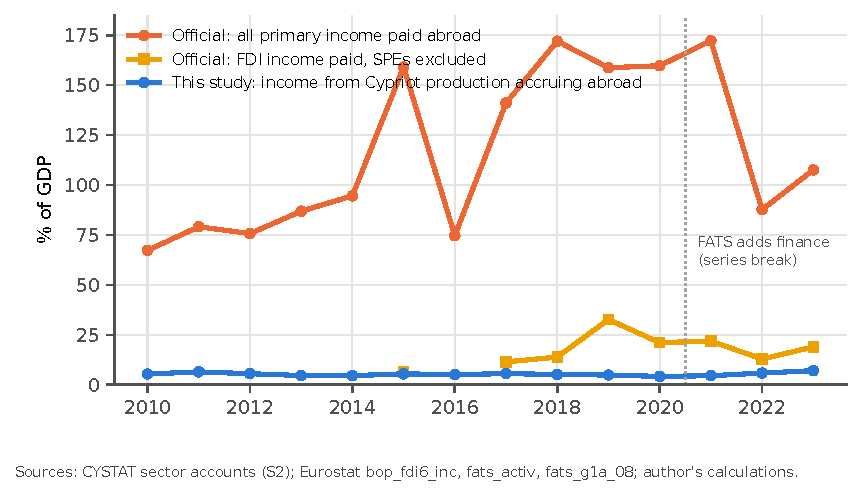
\includegraphics[width=\textwidth]{figures/official_vs_model.pdf}
\caption{Official primary income paid abroad versus income from Cypriot production accruing abroad, \% of GDP. The SPE-excluded FDI series starts in 2013 and has gaps where Eurostat marks cells confidential (2013--2014, 2016).}
\label{fig:official}
\end{figure}

\Cref{fig:official} shows the central result.
The official outflow---every euro of primary income paid to non-residents, including pass-through---moves between \OfficialOutMin{} and \OfficialOutMax{} of GDP.
FDI income paid excluding SPEs is far smaller but still volatile.
Income generated by Cypriot production that accrues abroad lies between \FVLMin{} and \FVLMax{} of GDP, and has risen since 2020.

\begin{figure}[!htbp]
\centering
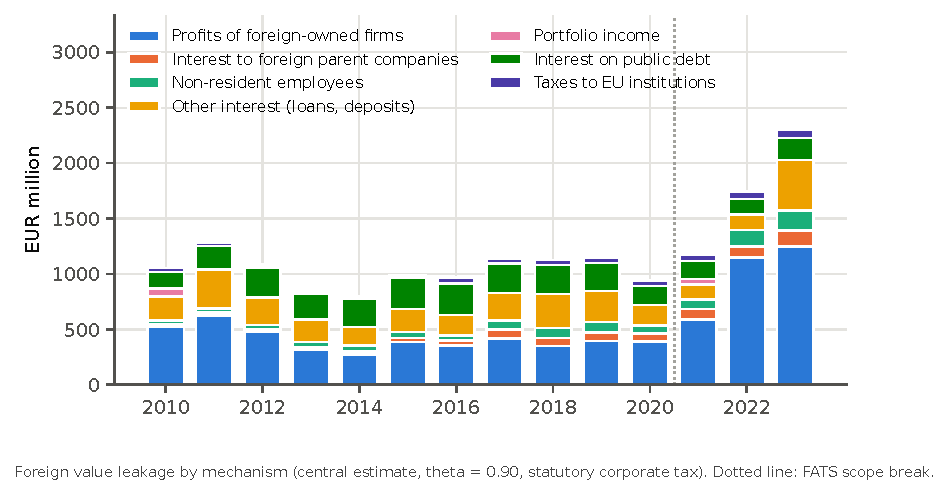
\includegraphics[width=\textwidth]{figures/mechanisms.pdf}
\caption{Value accruing abroad by mechanism, EUR million.}
\label{fig:mech}
\end{figure}

\Cref{fig:mech} decomposes the outflow.
Profits of foreign-owned firms are the largest mechanism (\MechFDIShare{} in \LastYear), and they drive the increase after 2020.
Pay to non-resident workers is small: \FLILast{} of compensation after employers' contributions.
Interest paid abroad on public debt peaked at \EUR\GovPeak~m in \GovPeakYear{}, fell to \EUR\GovTwentyTwo~m in 2022 and rose to \EUR\GovLast~m in \LastYear.
The 2021 step coincides with FATS adding finance and sections P--R.
With the same sections (B--N) in every year and banks from the balance of payments, retention in \LastYear{} is \DVRConsLast.

Two ratios summarise capital, both relative to the net operating surplus of all non-financial corporations, before interest and tax; the foreign-controlled numerator covers the same FATS sections (B--N) in every year.
Foreign-controlled firms, weighted by their non-resident equity share, account for \FOCLast{} of it in \LastYear{} (\FOCFirst{} in \FirstYear).
Because it is measured before interest, this share includes what those firms owe their lenders.
Part of its rise coincides with the 2021 switch of the FATS dataset, which roughly doubled measured foreign-controlled surplus in section J.
Interest and portfolio income that firms and banks paid to foreign lenders was equal in size to \FCredLast{} of the same surplus; the two ratios overlap and are not added.
These ratios have different bases from retention and are not added to it.

\section{From the official outflow to this estimate}
\label{sec:bridge}

\begin{table}[!htbp]
\centering
\footnotesize
\caption{From the official outflow to this study's estimate, 2023 (EUR m)}
\label{tab:bridge}
\setlength{\tabcolsep}{3pt}
\begin{tabular}{>{\raggedright\arraybackslash}p{0.34\textwidth}rr>{\raggedright\arraybackslash}p{0.40\textwidth}}
\toprule
Line (resident sector paying) & Official & This study & Reason for the difference \\
\midrule
1 Compensation of employees paid (S2 D1) & 230 & 182 & model is net of Cypriot employer social contributions \\
2 Taxes on production to EU institutions (S2 D2) & 74 & 74 & identical \\
3 Property income: NA (S2 D4) minus BoP total (S1) & 0 & 0 & vintage/compilation gap between national accounts and BoP \\
4 Non-bank financial corporations incl. SPEs (S12M) & 29,224 & 174 & excluded as pass-through, except the FATS profit of foreign-owned insurers and auxiliary financial firms (from 2021) \\
5 Central bank (S121) & 0 & 0 & excluded: reserve management \\
6 Banks (S122) & 1,500 & 640 & model: foreign-owned finance profit (FATS K from 2021; BoP bank FDI equity income before) + banks' interest net of receipts \\
7 General government (S13) & 197 & 197 & identical (interest items) \\
8a Firms and households: FDI equity income (S1V) & 2,633 & 610 & model uses FATS (production-based): the difference is income passed on by non-SPE holding and trading companies, plus FATS/BPM6 concept differences \\
8b Firms and households: FDI debt interest (S1V) & 572 & 145 & model caps intra-group interest at the interest deducted from foreign-controlled firms' surplus \\
8c Firms and households: other interest and portfolio income (S1V) & 457 & 456 & identical where published; confidential items omitted (lower bound) \\
Total & 34,887 & 2,478 & official primary income paid vs this study's outflow \\
\bottomrule
\end{tabular}

\smallskip
\begin{minipage}{0.95\textwidth}\footnotesize Notes: official = CYSTAT rest-of-world account (D1, D2, D4 received by the rest of the world) and the balance of payments by paying resident sector (Eurostat bop\_c6\_a). The official lines add up to the official total in every year 2010--2023; the full series is in \texttt{data/processed/bridge.parquet}.\end{minipage}
\end{table}


\Cref{tab:bridge} bridges the official outflow to our estimate by paying sector.
The largest line is income paid by non-bank financial corporations: \EUR\BridgeSpeLast~bn in \LastYear, almost all of it pass-through.
The second is FDI equity income paid by firms and households.
The balance of payments records \EUR\BridgeFdiEqOfficialLast~bn, while the FATS-based profit of foreign-controlled non-financial firms is \EUR\BridgeFdiEqModelLast~bn.
The \EUR\BridgeFdiEqGapLast~bn difference is income that holding and trading companies with staff receive from abroad and pass on, plus differences between the FATS and balance-of-payments concepts.
Our data cannot split these two components.
This line, not the SPE rule, explains most of the distance between the official figure and ours outside S12M.

Banks show the largest disagreement between two official sources.
In \LastYear{} the balance of payments records FDI equity income paid by banks of \EUR\BankBopLast~m, almost all of it reinvested earnings.
Our FATS-based profit of foreign-owned banks is \EUR\BankFatsLast~m, although the balance-of-payments figure is already after interest and tax and should, if anything, be smaller.
The two sources agree in 2021 and 2022 (within \EUR\BankAgreeGap~m) and diverge only in \LastYear{}, when bank profits jumped.
Our \EUR\BankFatsLast~m is the banks' share of FATS finance, which is published only as a whole; against all of finance the observed gap is smaller but still large.
Three explanations are possible, and published data cannot separate them; the timing fits best a large bank that the two sources classify differently.
FATS may treat Bank of Cyprus as domestically controlled, while the balance of payments treats all its profit as income of its Irish holding company.
The balance of payments also includes 10--50\% stakes, which FATS does not.
And the two sources may record provisions differently.
The central estimate uses FATS, the same source as every other industry, from 2021, and the balance of payments before 2021, when FATS does not cover finance: the series splices two sources that disagree in \LastYear{}.
The consistent-scope series (\DVRConsLast{} retention in \LastYear{}) uses the balance of payments throughout, and shows the same post-2020 decline.

\section{Industry decomposition}
\label{sec:industry}

\begin{table}[!htbp]
\centering
\small
\caption{Industry decomposition: GVA and retention 2023; input exposure 2022}
\label{tab:industries}
\begin{tabular}{>{\raggedright\arraybackslash}p{0.30\textwidth}rrrrr}
\toprule
Industry & GVA 2023 & \multicolumn{2}{c}{Input exposure 2022} & Foreign & Domestic \\
 & EUR m & direct & total & own. 2023 & retention 2023 \\
\midrule
Restaurants and accommodation & 1,829 & 25.0 & 25.1 & 1.8 & 97.1 \\
Retail & 1,383 & 31.6 & 18.8 & -- & 93.2 \\
Banking & 2,071 & 56.2 & 48.2 & -- & 68.5 \\
Insurance & 162 & 51.5 & 44.8 & -- & 80.5 \\
Telecommunications & 428 & 41.0 & 30.9 & -- & 88.0 \\
Energy & 349 & 49.7 & 48.6 & -- & 97.7 \\
Land transport & 200 & 45.5 & 37.1 & -- & 95.9 \\
Water transport (shipping) & 480 & 47.0 & 46.5 & -- & 93.2 \\
Construction & 1,595 & 20.1 & 37.0 & -- & 98.0 \\
Real estate (market) & 1,142 & 23.9 & 7.8 & -- & 95.9 \\
Professional services & 1,465 & 29.0 & 14.7 & -- & 95.4 \\
Manufacturing: food & 435 & 26.8 & 40.3 & -- & 96.2 \\
Technology (IT services) & 1,389 & 76.4 & 69.5 & 46.6 & 87.4 \\
Publishing incl. software & 1,124 & 71.8 & 62.2 & 37.5 & 79.8 \\
Auxiliary financial services & 703 & 81.3 & 67.8 & -- & 78.7 \\
Wholesale trade & 1,686 & 41.8 & 15.8 & -- & 91.1 \\
\bottomrule
\end{tabular}

\smallskip
\begin{minipage}{0.95\textwidth}\footnotesize
Notes: percentages. Direct foreign input exposure = imported share of the industry's intermediate inputs. Total = imports embodied in one euro of final demand for the product, through the whole supply chain (Leontief inverse); the two have different denominators and are not comparable by subtraction. Foreign ownership capture = foreign-owned net operating surplus before interest and corporate tax (FATS, after corporate depreciation, times theta) as a share of the industry's net operating surplus, which also includes self-employed income. Domestic retention = share of the industry's GVA accruing to residents. From 2021 FATS publishes finance (K), trade (G) and most of transport (H) only at section level, so industries within these sections share one foreign share. Recipient countries are not shown by industry: FATS publishes the ultimate controlling economy mostly for whole sections, so industry-by-country cells are fitted, not observed (see the dashboard, flagged low confidence).
\end{minipage}
\end{table}


\Cref{tab:industries} reports, for industries of policy interest and the largest ones, their GVA, foreign input exposure, foreign ownership capture and retention.
In \LastYear{} the largest outflows came from \IndOneName{} (\EUR\IndOneEUR~m; retention \IndOneDVR) and \IndTwoName{} (\EUR\IndTwoEUR~m; \IndTwoDVR).
Public administration retains almost all of its value added: it has little operating surplus to pay abroad.
FATS publishes finance only as a whole, so foreign-owned profit in finance is split between banking, insurance and auxiliary services in proportion to their operating surplus; the split is an allocation, not an observation.
Publishing (including software) and IT services are activities where intellectual property matters.
Their measured surplus may partly be profit shifted into Cyprus by multinational groups \citep{Guvenenetal2022}.
Conversely, intra-group service imports can move profit out as intermediate consumption, which Frame A cannot see.
For these industries ``value generated by production'' is an accounting label, not a statement about where the underlying activity takes place.

\section{Country decomposition}
\label{sec:country}

\begin{figure}[!htbp]
\centering
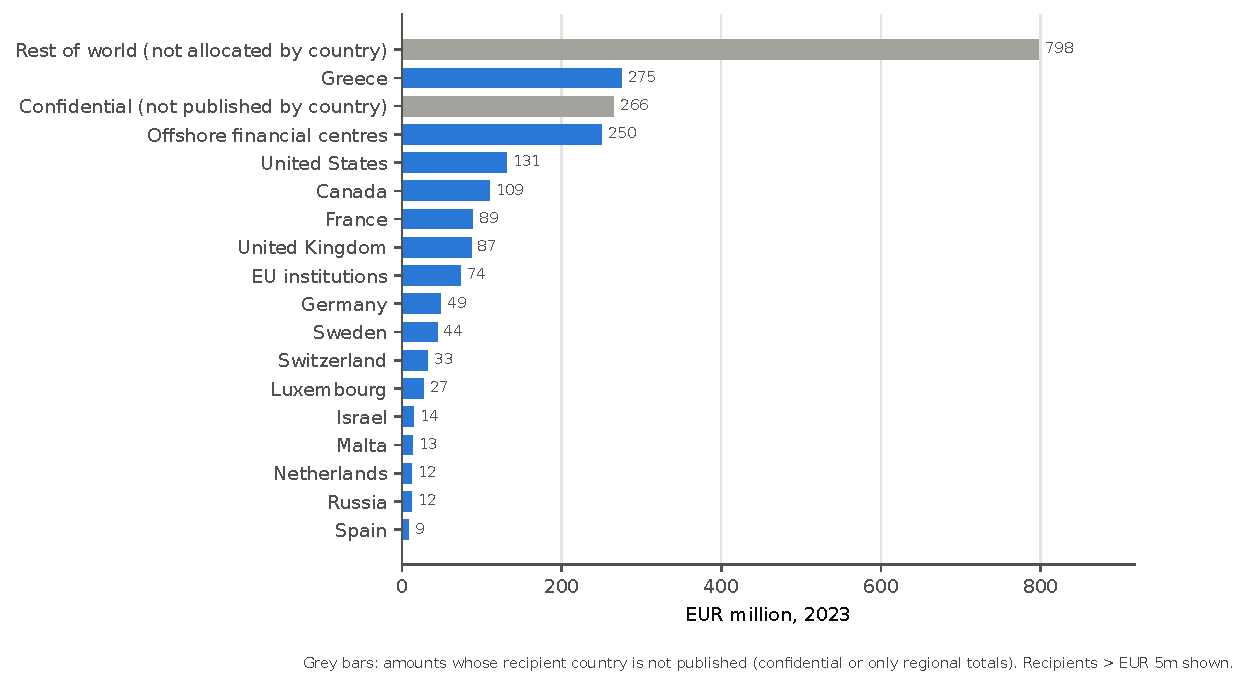
\includegraphics[width=0.95\textwidth]{figures/recipients_2023.pdf}
\caption{Recipients of value generated in Cyprus, \LastYear{}, EUR million, by ultimate controlling economy of the paying firm. Grey: country not published.}
\label{fig:recipients}
\end{figure}

\Cref{fig:recipients} answers the question ``to whom?''.
The country is that of the ultimate controlling unit of the paying firm.
For a listed parent, that is the parent's country, even though its shareholders may live anywhere.
Among identified recipients, \RecOneName{} (\EUR\RecOneEUR~m) and \RecTwoName{} (\EUR\RecTwoEUR~m) lead, followed by \RecThreeName{}, \RecFourName{} and \RecFiveName{}.
``Offshore financial centres'' is Eurostat's aggregate of offshore financial jurisdictions; it also contains operating economies such as Hong Kong, which we count only once, inside the aggregate.
When FATS names them as ultimate controller, the chain stops there; statistics cannot see who stands behind an offshore vehicle.
This is one reason why Russia, often discussed as a large investor in Cyprus, appears small as an ultimate controller of \emph{producing} firms.
Ireland does not appear as a named ultimate controller although the holding company of Bank of Cyprus is incorporated there.
FATS flags some Irish cells in 2021--2023, finance included, as confidential, while it publishes empty cells as zero, so Irish-controlled firms exist in Cypriot finance.
The published EU-controlled total less the published EU member cells shows that all confidential EU controllers of finance, Ireland included, together hold \EUR\IrishFinBoundFirst~m to \EUR\IrishFinBoundLast~m a year, net; this caps Irish-controlled finance only if none of the other confidential cells is negative.
We never assign a suppressed economy's total to a named country.
Within a country's published total, however, the split across sections is fitted where the section cell is suppressed; those rows are flagged as fitted and carry low confidence.
\EUR\RecUnknownEUR~m (\RecUnknownShare) cannot be assigned.
\EUR\RecConfEUR~m is suppressed for confidentiality, and \EUR\RecWorldEUR~m is interest paid by firms, households and the government that the balance of payments publishes only as a world total.

\section{Value chains: where does a euro of spending go?}
\label{sec:valuechain}

\begin{figure}[!htbp]
\centering
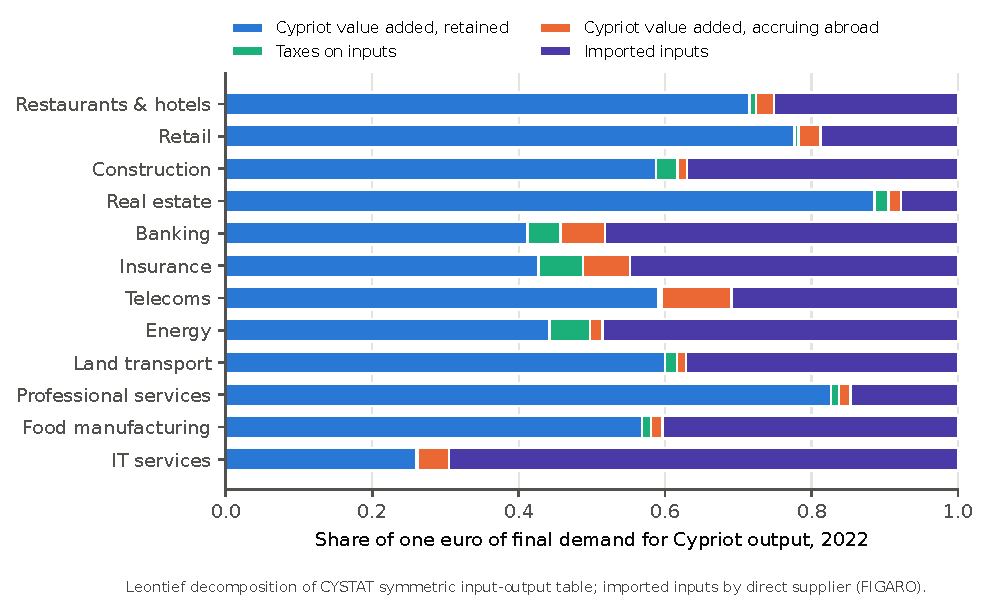
\includegraphics[width=\textwidth]{figures/per_euro_2022.pdf}
\caption{Where one euro of final demand for Cypriot output ends up, \IOLastYear{} (basic prices).}
\label{fig:pereuro}
\end{figure}

Frame B traces spending (\cref{fig:pereuro}).
Of a euro spent in restaurants and hotels, \PERestHome~cents are Cypriot value added that stays in Cyprus, \PERestAbroadVA~cents are Cypriot value added accruing to foreign owners, workers or lenders, and \PERestImp~cents buy imported inputs.
Retail keeps \PERetailHome~cents, construction \PEConstrHome, and market real estate \PERealEstHome.
IT services keep \PEITHome~cents: \PEITImp~cents of each euro buy imported inputs.
Across all final demand for Cypriot output in \IOLastYear{}, Cypriot value added was \EUR\EconDomVA~m (equal to GVA, an identity) and imported inputs \EUR\EconImp~m.
Among supplying countries, \ImpSrcOneName{} (\EUR\ImpSrcOneEUR~bn), \ImpSrcTwoName{} (\EUR\ImpSrcTwoEUR~bn) and \ImpSrcThreeName{} (\EUR\ImpSrcThreeEUR~bn) are the largest identified.
FIGARO's residual ``rest of the world'' block is larger still, and its bilateral services trade is partly modelled.
Russia's position as a leading supplier in 2022 reflects these modelled services flows and should be read with care.

\begin{figure}[!htbp]
\centering
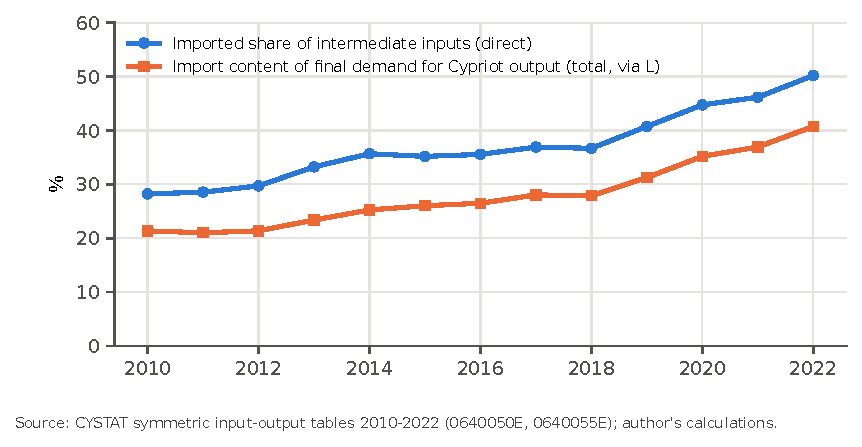
\includegraphics[width=\textwidth]{figures/input_exposure.pdf}
\caption{Foreign input exposure, direct and total, \FirstYear--\IOLastYear.}
\label{fig:fie}
\end{figure}

\Cref{fig:fie} shows that dependence on imported inputs rose steadily.
The largest increases are in IT services, banking, auxiliary financial services and publishing.

\paragraph{A worked example (illustrative).}
Return to the \EUR20 commission.
No accounts of the Cypriot subsidiary of the largest delivery platform are public.
We give the platform the average cost structure of Cyprus's information-services industry and the ownership chain in company filings: the Cypriot company is owned by a Finnish company, which is owned by a US-listed parent.
Most of the \EUR20 leaves Cyprus, but mainly as \emph{imports}, not as the owner's profit.
\EUR\PlatImp{} buys imported inputs such as software and cloud services, \EUR\PlatOwner{} is profit accruing to the US parent, and \EUR\PlatSuppAbroad{} is foreign income earned through Cypriot suppliers.
\EUR\PlatHome{} stays in Cyprus, including \EUR\PlatLabour{} of platform staff pay.
The import share comes from the industry average, which is dominated by large IT firms buying services from affiliates abroad; a delivery platform may differ.
The example is illustrative and is not part of any headline number.

\section{Robustness and sensitivity}
\label{sec:robust}

\begin{figure}[!htbp]
\centering
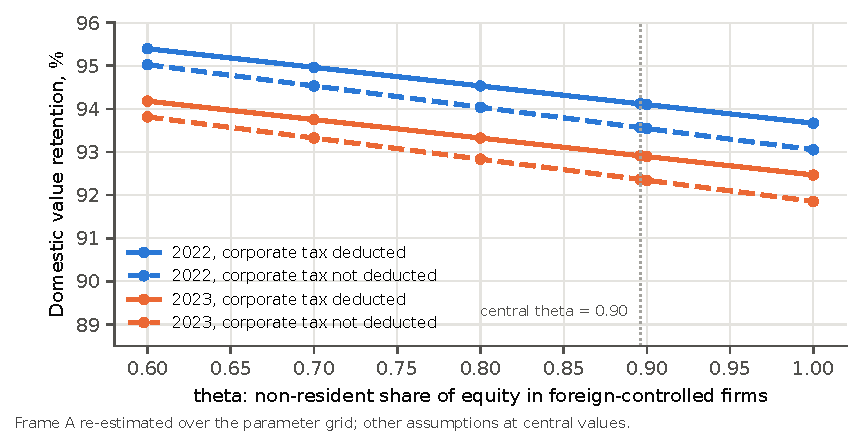
\includegraphics[width=\textwidth]{figures/sensitivity.pdf}
\caption{Domestic value retention under alternative $\theta$ and tax assumptions.}
\label{fig:sens}
\end{figure}

\Cref{fig:sens} varies the two unobserved parameters.
Moving $\theta$ from 0.6 to 1 changes \LastYear{} retention by \SensThetaSpreadPP{} percentage points.
Not deducting corporate tax gives \SensNoTaxDVR{}.
Using the FATS level of foreign-controlled finance surplus where it exceeds the national accounts gives \SensFatsLevelDVR{}.
Not deducting interest from foreign-controlled surplus gives \SensRhoNoneDVR{}; deducting interest net of receipts gives \SensRhoNetDVR{}; deducting actual interest before the bank-services adjustment gives \SensRhoGrossDVR{}.
Three variants test whether retention is overstated:
\begin{itemize}
\item counting banks' interest paid abroad gross, not net of receipts, and charging it to the borrowers whose loans it funds, gives \SensBanksGrossDVR{} in \LastYear{} and \SensBanksGrossFirst{} in \FirstYear{} (against \DVRFirst). Banks paid \EUR\BanksPaidFirst~m of such interest in \FirstYear{} and received \EUR\BanksRecvFirst~m;
\item taking foreign-owned profit from the balance of payments instead of FATS, an upper bound because that series includes pass-through by holding companies, gives \SensBopUpperDVR;
\item assigning the outflows of non-bank financial corporations to Cypriot production, capped at that industry's surplus, gives \SensOFCDVR.
\end{itemize}
Across all variants, \LastYear{} retention lies between \SensAllLow{} and \SensAllHigh.
In every variant, retention in \LastYear{} is below its 2020 level; the year-to-year path in between differs across variants.
Reconciliation is exact for GDP and compensation.
The official data satisfy the GNI identity to within \GNIMaxGap{}, which checks the data we use, not the model.

\section{Cyprus among other small open economies}
\label{sec:compare}

Is \DVRLast{} a lot or a little?
To answer, we run the same estimator on five other euro-area economies: three that also host many foreign firms (Ireland, Luxembourg, the Netherlands) and two that do not (Greece, Portugal).
Nothing in the method changes, only the sources.
The rest-of-world account comes from Eurostat instead of CYSTAT, and the tax rate from the OECD.
Run on Cyprus with the Eurostat sources, the estimator reproduces every mechanism to within the rounding of the two publications.
Three caveats apply.
First, $\theta$ is calibrated only for Cyprus, so elsewhere it is an assumption, and we also show $\theta=1$; the two differ by at most \CmpThetaMaxGap{} points.
Second, where a country suppresses an input we coarsen or skip, and never fill it in.
Malta could not be included because it never publishes mining and energy separately.
Third, from 2021 FATS covers finance in every country, so in the hubs years before and after 2021 are not comparable; we compare countries within a year.

\begin{table}[!htbp]
\centering
\small
\caption{Domestic value retention in Cyprus and five EU economies (\% of GDP)}
\label{tab:comparison}
\begin{tabular}{lrrrrr>{\raggedright\arraybackslash}p{0.27\textwidth}}
\toprule
 & \multicolumn{3}{c}{Retention, Cyprus $\theta$} & $\theta=1$ & Official & Largest outflow \\
\cmidrule(lr){2-4}
Country & 2015 & 2019 & 2023 & 2023 & outflow 2023 & line, 2023 \\
\midrule
Cyprus & 94.5 & 95.1 & 92.9 & 92.5 & 107.5 & foreign-owned profit (3.8) \\
Ireland & 79.8 & 78.6 & 71.7 & 69.2 & 73.9 & foreign-owned profit (21.9) \\
Luxembourg & 80.6 & 79.0 & 74.0 & 73.1 & 442.8 & non-resident employees (17.5) \\
Netherlands & 92.3 & -- & 92.8 & 92.5 & 38.7 & foreign-owned profit (2.7) \\
Greece & 96.3 & 96.2 & 95.4 & 95.2 & 7.1 & public debt interest (2.2) \\
Portugal & 94.6 & 95.5 & 95.4 & 95.1 & 8.2 & foreign-owned profit (2.8) \\
\bottomrule
\end{tabular}

\smallskip
\begin{minipage}{0.95\textwidth}\footnotesize Notes: Frame A with the Cyprus method; other countries from Eurostat (\texttt{nasa\_10\_nf\_tr}, \texttt{nama\_10\_a64}, FATS, \texttt{bop\_c6\_a}, \texttt{bop\_rem6}) and OECD statutory tax rates. $\theta$ is calibrated for Cyprus only and assumed elsewhere; $\theta=1$ gives the lowest retention. Official outflow: primary income paid abroad (S2), which includes pass-through income. -- = inputs suppressed (Netherlands 2019). Malta is omitted in every year (sections B, D not published separately in the national accounts). From 2021 FATS covers finance; before, foreign-owned banks' profit comes from the balance of payments, so columns before and after 2021 differ in scope. Suppressed balance-of-payments items are omitted (a suppressed bank receipt is not netted): Cyprus: portfolio dividends (firms and households) (2015, 2019, 2023), portfolio dividends (banks, received) (2015, 2019, 2023); Ireland: portfolio dividends (firms and households) (2015, 2019), portfolio dividends (banks, received) (2019, 2023); Luxembourg: foreign-owned banks' profit (banks) (2015, 2019), loan and deposit interest (firms and households) (2015, 2019, 2023), portfolio dividends (firms and households) (2015, 2019, 2023), policyholder income (firms and households) (2015, 2019, 2023), intra-group interest (firms and households) (2015, 2019, 2023), loan and deposit interest (banks) (2015, 2019, 2023), portfolio dividends (banks) (2015, 2019, 2023), policyholder income (banks) (2015, 2019, 2023), loan and deposit interest (banks, received) (2015, 2019, 2023), portfolio dividends (banks, received) (2015, 2019, 2023), policyholder income (banks, received) (2015, 2019, 2023), loan and deposit interest (government) (2015, 2019, 2023); Greece: foreign-owned banks' profit (banks) (2015, 2019).\end{minipage}
\end{table}


\Cref{tab:comparison} shows three different ways to leak value.
In Ireland, \CmpIEProfit{} of GDP in \CmpYear{} is profit of foreign-controlled firms, mostly in manufacturing and information and communication, and retention is \CmpIE.
In Luxembourg, the largest line, \CmpLUCommuters{} of GDP, is pay to employees who live in France, Belgium and Germany.
They are non-residents, so their pay leaves the economy.
Their nationality plays no part in this; where they live is what counts.
Luxembourg's retention of \CmpLU{} is overstated: much of the interest and dividends paid abroad by its firms, households, banks and government is confidential and therefore missing.
In Greece (\CmpEL), the largest line is interest on public debt held abroad, \CmpELPublic{} of GDP.

The official outflow column is the reason for this exercise.
Primary income paid abroad is \CmpLUOfficial{} of GDP in Luxembourg, \OfficialOutLast{} in Cyprus, \CmpIEOfficial{} in Ireland and \CmpNLOfficial{} in the Netherlands.
Most of it is income passing through holding companies and funds, so the official ratio says little about value retained.
Ireland has a lower official ratio than Cyprus but retains much less, and the Netherlands a lower ratio than Cyprus and retains about as much.
Cyprus retains about as much as the Netherlands (\CmpNL), less than Portugal (\CmpPT) and Greece, and at least \CmpHubGap{} points more than Ireland and Luxembourg.

\section{Limitations}
\label{sec:limits}

The full list, with the data that would remove each limitation, is in the repository's limitations file.
The most important are these.
(i) Retention is an upper bound.
Outflows we cannot measure count as retained: rent earned by non-resident owners of Cypriot dwellings, and FDI income from stakes of 10--50\% in domestically controlled firms.
(ii) Before 2021, foreign-owned insurers and auxiliary financial firms are missing.
In 2021, their first year, they accounted for about \InsAuxShareFirstFats{} of GDP (an allocated share of FATS finance).
(iii) $\theta$ is calibrated on documented large firms, not measured.
(iv) Excluding non-bank financial corporations is a sector rule, not an entity-level SPE flag.
(v) Residence follows incorporation, so a Cypriot bank whose holding company is incorporated in Ireland is Irish-controlled at company level, although its shareholders include Cypriots.
(vi) FATS operating surplus and national-accounts operating surplus differ in concept (treatment of financial intermediation services, software and research, statistical units), and the interest deduction is not applied to finance.
(vii) Imports are attributed to the direct supplier.

\section{Discussion}
\label{sec:discussion}

The headline---Cyprus retains at most \DVRLast{} of the value it produces---is less dramatic than the official outflow and more informative.
It separates two things that official aggregates mix.
One is Cyprus as a financial conduit, through which foreign income flows of the order of GDP (between two-thirds of GDP and 1.7 times GDP a year).
The other is Cyprus as a producing economy, where foreign-controlled firms account for \FOCLast{} of non-financial corporate operating surplus before interest and tax, a share that has grown since 2020.
Adding a country is a data run, not a new model: every Eurostat input exists for all EU member states, and the only Cyprus-specific loader, for sector accounts, has a Eurostat equivalent.

\section{Conclusion}
\label{sec:conclusion}

Of the value generated in Cyprus in \LastYear{}, at most \DVRLast{} accrued to residents and at least \FVLLast{} to the rest of the world.
Most of what accrued abroad was profits of foreign-owned firms, with \RecOneName{}, \RecTwoName{}, \RecThreeName{} and \RecFourName{} as the largest identified recipients.
Official primary-income outflows, at \OfficialOutLast{} of GDP, measure something else: the traffic of a financial hub.
Every number above can be traced in the accompanying database and dashboard, from the headline through industry, mechanism and source table to the calculation that produced it.

\bibliographystyle{plainnat}
\bibliography{references}

\appendix
\section{Data appendix}
\label{app:data}
Every dataset is listed in \texttt{data\_catalogue.csv} with provider, URL, reference period, publication and download dates, licence, scope, resolution, variables, processing script and SHA-256 checksum. Raw files are not redistributed; \texttt{make ingest} downloads them again, and checksums confirm that the same vintage is used.

\begin{table}[h]
\centering
\small
\caption{Datasets in the catalogue by provider}
\label{tab:catalogue}
\begin{tabular}{lr}
\toprule
Provider & Datasets \\
\midrule
CYSTAT (Statistical Service of Cyprus) & 43 \\
Central Bank of Cyprus & 8 \\
Compiled from company filings (Tier 1-4, per row) & 1 \\
Eurostat & 44 \\
\bottomrule
\end{tabular}
\end{table}


\section{Methodological appendix}
\label{app:method}
\begin{table}[!htbp]
\centering
\small
\caption{Depreciation, interest and intra-group share per euro of non-financial corporations' surplus}
\label{tab:rho}
\begin{tabular}{lrrrrr}
\toprule
Year & $c$ & $\rho$ (central) & $\rho$ net & $\rho$ pre-FISIM & $s$ \\
\midrule
2010 & 0.34 & 0.34 & 0.29 & 0.67 & 0.17 \\
2011 & 0.34 & 0.38 & 0.33 & 0.66 & 0.17 \\
2012 & 0.38 & 0.33 & 0.28 & 0.70 & 0.19 \\
2013 & 0.38 & 0.35 & 0.27 & 0.72 & 0.17 \\
2014 & 0.43 & 0.34 & 0.23 & 0.74 & 0.21 \\
2015 & 0.41 & 0.45 & 0.33 & 0.76 & 0.17 \\
2016 & 0.34 & 0.36 & 0.28 & 0.55 & 0.21 \\
2017 & 0.32 & 0.30 & 0.25 & 0.48 & 0.40 \\
2018 & 0.30 & 0.28 & 0.25 & 0.42 & 0.37 \\
2019 & 0.30 & 0.28 & 0.21 & 0.41 & 0.41 \\
2020 & 0.34 & 0.27 & 0.21 & 0.45 & 0.42 \\
2021 & 0.29 & 0.19 & 0.13 & 0.31 & 0.49 \\
2022 & 0.26 & 0.12 & 0.07 & 0.20 & 0.57 \\
2023 & 0.26 & 0.27 & 0.19 & 0.21 & 0.33 \\
\bottomrule
\end{tabular}

\smallskip
\begin{minipage}{0.9\textwidth}\footnotesize Notes: ratios to S11 gross operating surplus (Eurostat \texttt{nasa\_10\_nf\_tr}). Central $\rho$ = interest paid after the FISIM adjustment; net = paid minus received; pre-FISIM = actual interest paid. $s$ = FDI debt interest paid by firms and households (BoP) / S11 interest paid.\end{minipage}
\end{table}

\begin{table}[h]
\centering
\small
\caption{Reconciliation with official aggregates}
\label{tab:recon}
\begin{tabular}{>{\raggedright\arraybackslash}p{0.5\textwidth}lrrc}
\toprule
Check & Years & Max $|$diff.$|$ \% & Tol. \% & Pass \\
\midrule
Compensation of employees (SIOT vs sector accounts S1 D1 paid) & 2010--2022 & 0.0001 & 0.50 & \checkmark \\
GDP = sum of GVA + taxes less subsidies on products & 2010--2022 & 0.0002 & 0.50 & \checkmark \\
GNI = GDP + primary income received - primary income paid (rest of world) & 2010--2024 & 0.0077 & 0.10 & \checkmark \\
Recipient tensor sums to GDP & 2010--2023 & 0.0005 & 0.50 & \checkmark \\
\bottomrule
\end{tabular}

\smallskip
\begin{minipage}{0.9\textwidth}\footnotesize Notes: official values from CYSTAT annual national accounts (April 2026 vintage) and sector accounts; model values from the input--output tables and the recipient accounting. Residuals are reported, not forced to zero.\end{minipage}
\end{table}

The validation suite (\texttt{python -m cvr.validate}) runs after every model build and exits with an error if any check fails. In this release 30 of 30 checks pass; unit tests add further guards on synthetic data.

\begin{table}[h]
\centering
\small
\caption{Automated validation checks}
\label{tab:validation}
\begin{tabular}{>{\raggedright\arraybackslash}p{0.75\textwidth}c}
\toprule
Check & Pass \\
\midrule
{}[identity] tensor sums to GDP every year & \checkmark \\
{}[identity] industry rows sum to GVA (all years) & \checkmark \\
{}no negative outflows & \checkmark \\
{}no negative unexplained retained flows & \checkmark \\
{}[identity] DVR + FVL = 1 & \checkmark \\
{}0 <= FVL <= 1 & \checkmark \\
{}[identity] Frame B: each euro sums to 1 & \checkmark \\
{}[identity] Frame B: domestic VA of all final demand = GVA & \checkmark \\
{}Frame B: imported inputs counted once (= total imported intermediates) & \checkmark \\
{}IO: VA + import + tax content = 1 (every product, every year) & \checkmark \\
{}IO: direct import share within [0,1] & \checkmark \\
{}ownership: no duplicate edges, shares <= 100\% & \checkmark \\
{}ownership: ultimate shares sum to 100\% per firm & \checkmark \\
{}reconciliation: all checks within tolerance & \checkmark \\
{}provenance complete on all tables & \checkmark \\
{}intra-group interest only on industries with foreign-controlled surplus & \checkmark \\
{}source: creditor share = firms' and banks' interest abroad / S11 NOS & \checkmark \\
{}fitted-cell flag and low confidence exactly where the FATS cell is suppressed & \checkmark \\
{}source: banks' interest = max(BoP paid - received, 0) & \checkmark \\
{}source: households' loan interest on imputed rent = their D41 share x S1V loan interest & \checkmark \\
{}source: every FATS row = base x (1 - CFC - interest) x (1 - tau) x theta (raw S11/S12 ratios) & \checkmark \\
{}theta used = theta recalibrated from the company layer & \checkmark \\
{}source: intra-group interest = min(BoP FDI debt interest, s x interest deducted) & \checkmark \\
{}source: non-resident pay = S2 D1 x (1 - employer SSC share) & \checkmark \\
{}source: EU taxes = S2 D2 & \checkmark \\
{}source: public-debt interest = BoP S13 interest paid & \checkmark \\
{}source: FATS base of foreign-owned profit = published FATS total (less losses) & \checkmark \\
{}source: foreign-owned banks counted once (BoP before 2021, FATS K from 2021) & \checkmark \\
{}bridge: official lines add up to official outflow; model lines to model outflow & \checkmark \\
{}time-series breaks identified and documented & \checkmark \\
\bottomrule
\end{tabular}
\end{table}


\end{document}
